
%packages
\usepackage{natbib}
\usepackage{amsmath}
\usepackage{amsthm}
\usepackage{mathtools}
\usepackage{mdframed}
\usepackage{subfigure}
\usepackage{booktabs}
% \usepackage{hyperref}
\usepackage{subfigure}
\usepackage{siunitx} % Provides the \SI{}{} and \si{} command for typesetting SI units
\usepackage{graphicx} % Required for the inclusion of images
% \usepackage{natbib} % Required to change bibliography style to APA
\usepackage{datetime}
\usepackage{lscape}
\usepackage{algorithm}
\usepackage{algorithmic}
\usepackage{xspace}
\usepackage[english]{babel} % English language/hyphenation
\usepackage{proof}
\usepackage{booktabs} % Top and bottom rules for tables
\usepackage[colorlinks, allcolors = blue,]{hyperref}
\usepackage{accents}
\usepackage{amsfonts}
\usepackage{stmaryrd}
\usepackage{amsmath,amsthm,amssymb,latexsym} 
\usepackage{microtype}
\usepackage{graphicx}
\usepackage{subfigure}
\usepackage{booktabs} % for professional tables
\usepackage{hyperref}
\usepackage{icml2019}
\usepackage{lipsum}

\usepackage{authblk}


%new commands
\newcommand{\theHalgorithm}{\arabic{algorithm}}
\newtheorem{definition}{Definition}
\usepackage{cancel}
\usepackage[normalem]{ulem}
\newcommand{\dataobs}{\textbf{x}}
\newcommand{\adj}[2]{\textbf{adj}(#1,#2)}
\newcommand{\candidateset}{\mathcal{R}_{\textup{post}}}
\newcommand{\bprior}{\boldsymbol{\beta}_{\textup{prior}}}
\newcommand{\bysinfer}{\mathsf{Infer}}
\newcommand{\betad}{\mathsf{Beta}}
\newcommand{\betaf}{\textup{B}}
\newcommand{\mbetaf}{\boldsymbol{\textup{B}}}
\newcommand{\vtheta}{\boldsymbol{\theta}}
\newcommand{\valpha}{\boldsymbol{\alpha}}
\newcommand{\vbeta}{\boldsymbol{\beta}}
\newcommand{\lapmech}{\mathsf{LSDim}}
\newcommand{\ilapmech}{\mathsf{LSHist}}
\newcommand{\binomial}[2]{\mathsf{Bin}(#1, #2)}
\newcommand{\multinomial}[2]{\mathsf{Mult}(#1, #2)}
\newcommand{\expmech}{\mathsf{EHD}}
\newcommand{\hexpmech}{\mathsf{EHDS}}
\newcommand{\lexpmech}{\mathsf{EHDL}}
\newcommand{\hexpmechd}{\mathsf{expMech}^{D}_{\hellinger}}
\newcommand{\privinfer}{\mathsf{PrivInfer}}
\newcommand{\hlg}{\mathsf{H}}
\newcommand{\dirichlet}[1]{\mathsf{Dir}(#1)}
\newcommand{\alphas}{\boldsymbol{\alpha}}
\newcommand{\xis}{\boldsymbol{\xi}}
\newcommand{\iverson}[1]{[#1]}
\newcommand{\datauni}{\mathcal{X}}
\newcommand{\hellinger}{\mathcal{H}}
\newcommand{\ux}[1]{u(\textbf{x}, {#1})}
\newcommand{\uxadj}[1]{u(\textbf{x}', {#1})}
\newcommand{\cardinality}[2]{\mathcal{C}^{#1}_{#2}}
\newcommand{\range}{\mathcal{O}}
\newcommand{\nomalizer}[1]{\sum\limits_{r'\in \mathcal{R}_{\textup{post}}} \exp \big(\frac{-\epsilon\cdot \mathcal{H} (\mathsf{BI}(#1),r')}{4 \cdot S(#1)}\big)}

\newcommand{\unomalizer}[1]{\sum\limits_{r'\in \mathcal{R}_{\textup{post}}} \exp \big(\frac{-\epsilon\cdot u(#1, r')}{4 \cdot S(#1)}\big)}


\newcommand{\hexpmechPr}[2]{\underset{z \thicksim \hexpmech(#1)}{\Pr}\left[ #2 \right]}
\newcommand{\lapmechPr}[2]{\underset{z \thicksim \lapmech(#1)}{\Pr}\left[ #2 \right]}

\newcommand{\ilapmechPr}[2]{\underset{
{z \thicksim \ilapmech(#1)}
}{\Pr}\left[ #2 \right]}

\newtheorem{thm}{Theorem}[section]

\newtheorem{lem}{Lemma}[section]

\newtheorem{assert}{Assertion}[lem]
\newcommand{\lap}[2]{\mathsf{Lap}(#1, #2)}
\newcommand{\todo}[1]{{\footnotesize \color{red}\textbf{[[ #1 ]]}}}

\title{\textbf{Notes of DP - Bayesian Inference}\\}
% \author{Jiawen \textsc{Liu}}
\date{\vspace{-10ex}}

\begin{document}
\maketitle

\section{Problem Statement}

\section{Technical Problem Statement}
\label{sec_bayesInfer}

Our technical problem is based on the Bernoulli-Beta Bayesian inference. In the Bayesian inference, first there is a prior distribution $\pi(\xis)$ to present our belief about parameter $\xis$. Then, we get some observed data $x$ sizing $n$, and produce a posterior distribution $Pr(\xis | x)$. The Bayesian inference is based on the Bayes' rule to calculate the posterior distribution:
\begin{equation*}
Pr(\xis | x) = \frac{Pr(x | \xis) \pi(\xis)}{Pr(x)}
\end{equation*}
It is denoted as $\bysinfer(x,\pi(\xis))$ taking an observed data set $x \in \mathcal{X}^n$ and a prior distribution $\pi(\xis)$ as input, outputting a posterior distribution of the parameter $\alphas$. For conciseness, when prior is given, we use $\bysinfer(x)$. $n$ is the size of the observed data size.

In our inference algorithm, we take a Dirichlet distribution as prior belief for the parameters, $\dirichlet(\alphas)$, where $\pi(\xis) = \dirichlet(\xis | \alphas) = \frac{\prod_{i = 1}^{m}\xi_i^{\alpha_i}}{B(\alphas)}$, and the Bernoulli distribution as the statistic model for $Pr(x | \alphas)$. $m$ is the order of the Dirichlet distribution.

We give a inference process based on a concrete example, where we throw an irregular $m$ sides dice. We want to infer the probability of getting each side $\xis$. We get a observed data set $\{s_{k_1}, s_{k_2}, \cdots, s_{k_n}\}$ by throwing the dice $n$ times, where $k_i \in \{1,2,\cdots, m\}$ denotes the side we get when we throw the dice the $i^{th}$ time. The posterior distribution is still a Dirichlet distribution with parameters $(\alpha_1 + n_1, \alpha_2 + n_2, \cdots, \alpha_m + n_m)$, where $n_i$ is the appearance time of the side $i$ in total.

In the case that $m = 2$, it is reduced to a Beta distribution $\betad(\alpha, \beta)$. The $m$ side dice change into a irregular coin with side $A$ and side $B$. The posterior is computed as $(\alpha + n_1, \beta + n_0)$, where $n_1$ is the appearance time of side $A$ in the observed data set and $n_0$ is the appearance time of the other side.

\section{Baseline Approach}

\section{Our Approach - Exponential Mechanism with Smooth Sensitivity}
\label{sec_smoo}

\subsubsection{Algorithm Setting up}
We define a new mechanism $\hexpmech(x)$
which is similar to the exponential mechanism where we use
$\mathcal{R}$ as the set $\betaset$ of beta distributions with integer parameters
summing up to $n+2$, as scoring function we use the Hellinger distance
from $\bysinfer(x)$, i.e. $\hlg(\bysinfer(x),-)$, and we 
calibrate the noise to the smooth sensitivity~\cite{nissim2007smooth}. The
only difference is in the sensitivity part, since now we use the
smooth sensitivity.

\begin{definition}
\label{def_smoo}
The mechanism $\hexpmech(x)$ outputs a candidate $r \in \betaset$ with probability
\begin{equation*}
\underset{z \thicksim \hexpmech(x)}{Pr}[z=r] = \frac
{exp(\frac{-\epsilon\hlg(\bysinfer(x),r)}{2 S_\beta(x)})}
{\Sigma_{r' \in R}\ exp(\frac{-\epsilon \hlg(\bysinfer(x),r')}{2 S_\beta(x)})},
\end{equation*}
where $s_\beta(x)$ is the smooth sensitivity of $\hlg(\bysinfer(x),-)$, calculated by:
\begin{equation*}
S_{\beta}(x) = \max(\Delta_{l}\hlg(\bysinfer(x),-), \max_{y \neq x; y \in D^{n}}(\Delta_{l}\hlg(\bysinfer(y),-)\cdot e^{-\beta d(x,y)})),
\end{equation*}
where $d$ is the Hamming distance between two datasets, and $\beta =
\beta(\epsilon, \delta)$ is a function of $\epsilon$ and $\delta$. 
\end{definition}


In what follows, we will use a correspondence between the probability
 $\underset{z \thicksim \hexpmech(x)}{Pr}[z = r]$ of every
 $r\in\betaset$ and the probability 
 $\underset{z \thicksim \hexpmech(x)}{Pr}[\hlg(\bysinfer(x),z) =
 \hlg(\bysinfer(x),r)]$ for the utility score for $r$. In particular, for every
 $r\in\betaset$ we have:
$$
\underset{z \thicksim \hexpmech(x)}{Pr}[z = r]=
\frac{1}{2}\Big (\underset{z \thicksim \hexpmech(x)}{Pr}[\hlg(\bysinfer(x),z) =
 \hlg(\bysinfer(x),r)]\Big )
$$
To see this, it is enough to notice that: $\underset{z \thicksim \hexpmech(x)}{Pr}[z = r]$ is proportional too $\hlg(\bysinfer(x),r)$, i.e., $u(x,z)$. We can derive, if $u(r,x) = u(r',x)$ then $\underset{z \thicksim \hexpmech(x)}{Pr}[z = r] = \underset{z \thicksim \hexpmech(x)}{Pr}[z = r']$. We assume the number of candidates $z \in \mathcal{R}$ that satisfy $u(z,x) = u(r,x)$ is $|r|$, we have  $\underset{z \thicksim \hexpmech(x)}{Pr}[u(z,x) = u(r,x)] = |r| \underset{z \thicksim \hexpmech(x)}{Pr}[z = r]$. Because Hellinger distance  $\hlg(\bysinfer(x),z)$ is axial symmetry, where the $\bysinfer(x)$ is the symmetry axis. It can be infer that $|z| = 2$ for any candidates, apart from the true output, i.e., $\underset{z \thicksim \hexpmech(x)}{Pr}[u(z,x) = u(r,x)] = 2 \underset{z \thicksim \hexpmech(x)}{Pr}[z = r]$. This parameter can be eliminate in both sides in proof.

In our private Bayesian inference mechanism, we set the $\beta$ as $\ln(1 - \frac{\epsilon}{2 \ln (\frac{\delta}{2 (n + 1)})})$. 





\subsubsection{Sliding Property of Exponential Mechanism}
\begin{lem}
Consider the exponential mechanism  $\sexpmech(x,u,\mathcal{R})$
calibrated on the smooth sensitivity. Let $\lambda = f(\epsilon,
\delta)$, $\epsilon\geq 0$ and $|\delta| < 1$. Then, the following \emph{sliding property} holds:
\begin{equation*}
\underset{r \thicksim \hexpmech(x)}{Pr}[u(r,x) = \hat{s}]
\leq
e^{\frac{\epsilon}{2}} \underset{r \thicksim \hexpmech(x)}{Pr}[u(r,x) = (\Delta + \hat{s})] + \frac{\delta}{2},
\end{equation*}

\end{lem}

\begin{proof}

We denote the normalizer of the probability mass in $\hexpmech(x)$: $\sum_{r' \in \mathcal{R}}exp(\frac{\epsilon u(r',x)}{2 S(x)})$ as $NL(x)$:
\begin{equation*}
\begin{split}
LHS 
  = \underset{r \thicksim \hexpmech(x)}{Pr}[u(r,x) = \hat{s}]
& = \frac{exp(\frac{\epsilon \hat{s}}{2 S(x)})}{NL(x)}\\
& = \frac{exp(\frac{\epsilon (\hat{s} + \Delta - \Delta)}{2 S(x)})}{NL(x)}\\
& = \frac{exp(\frac{\epsilon (\hat{s} + \Delta)}{2 S(x)} + \frac{- \epsilon \Delta}{2 S(x)})}{NL(x)}\\
& = \frac{exp(\frac{\epsilon (\hat{s} + \Delta)}{2 S(x)})}{NL(x)} \cdot e^{\frac{- \epsilon \Delta}{2 S(x)})}.\\
\end{split}
\end{equation*}

By bounding the $\Delta \geq -S(x)$, we can get:

\begin{equation*}
\begin{split}
\frac{exp(\frac{\epsilon (\hat{s} + \Delta)}{2 S(x)})}{NL(x)} \cdot e^{\frac{- \epsilon \Delta}{2 S(x)}}
& \leq \frac{exp(\frac{\epsilon (\hat{s} + \Delta)}{2 S(x)})}{NL(x)} \cdot e^{\frac{\epsilon}{2}}\\
&  =  e^{\frac{\epsilon}{2}} \underset{z \thicksim \hexpmech(x)}{Pr}[u(r,x) = (\Delta + \hat{s})] \leq RHS\\
\end{split}
\end{equation*}

\end{proof}

\subsubsection{Dilation Property of Exponential Mechanism}
\begin{lem}
for any exponential mechanism $\hexpmech(x)$, $\lambda < |\beta|$, $\epsilon$, $|\delta| < 1$ and $\beta \leq \ln(1 - \frac{\epsilon}{2 \ln (\frac{\delta}{2 (n + 1)})})$, the dilation property holds:

\begin{equation*}
\underset{z \thicksim \hexpmech(x)}{Pr}[u(z,x) = c]
\leq
e^{\frac{\epsilon}{2}} \underset{z \thicksim \hexpmech(x)}{Pr}[u(z,x) = e^{\lambda} c] + \frac{\delta}{2},
\end{equation*}
where the sensitivity in mechanism is still smooth sensitivity as above.
\end{lem}

\begin{proof}

The sensitivity is always greater than 0, and our utility function $-\hlg(\bysinfer(x),z)$ is smaller than zero, i.e., $u(z,x) \leq 0$, we need to consider two cases where $\lambda < 0$, and $\lambda > 0$:

We set the $h(c) = Pr[u(\hexpmech(x)) = c] = 2\frac{exp(\frac{\epsilon z}{2 S(x)})}{NL(x)}$.

We first consider $\lambda < 0$. In this case, $1 < e ^ {\lambda}$, so the ratio $\frac{h(c)}{h(e^{\lambda}c)} = \frac{exp(\frac{\epsilon c}{2 S(x)})}{exp(\frac{\epsilon (c \cdot e^{\lambda})}{2 S(x)})}$ is at most $\frac{\epsilon}{2}$.

Next, we proof the dilation property for $\lambda > 0$, The ratio of $\frac{h(c)}{h(e^{\lambda}c)}$ is $\exp(\frac{\epsilon}{2} \cdot \frac{u(\hexpmech(x)) (1 - e^{\lambda})}{S(x)})$. Consider the event $G = \{ \hexpmech(x) : u(\hexpmech(x)) \leq \frac{S(x)}{(1 - e^{\lambda})}\}$. Under this event, the log-ratio above is at most $\frac{\epsilon}{2}$. The probability of $G$ under density $h(c)$ is $1 - \frac{\delta}{2}$. Thus, the probability of a given event $z$ is at most $Pr[c \cap G] + Pr[\overline{G}] \leq e^{\frac{\epsilon}{2}} Pr[e^{\lambda}c \cap G] + \frac{\delta}{2} \leq e^{\frac{\epsilon}{2}} Pr[e^{\lambda}c] + \frac{\delta}{2}$.\\


\textbf{Detail proof:}
\begin{itemize}

	\item $\lambda < 0$

		The left hand side will always be smaller than 0 and the right hand side greater than 0. This will always holds, i.e.
		\begin{equation*}
		\end{equation*}
	\item $\lambda > 0$


Because $\hat{s} = u(r)$ where $r \thicksim \hexpmech(x)$, we can substitute $\hat{s}$ with $u(\hexpmech(x))$. Then, what we need to proof under the case $\lambda > 0$ is:
\begin{equation*}
u(\hexpmech(x)) \leq \frac{S(x)}{(1 - e ^ {\lambda})}
\end{equation*}
By applying the accuracy property of exponential mechanism, we bound the probability that the equation holds with probability:
\begin{equation*}
\begin{split}
Pr[u(\hexpmech(x)) \leq \frac{S(x)}{(1 - e ^ {\lambda})}] 
& \leq \frac{|\mathcal{R}|exp(\frac{\epsilon S(x)}{(1 - e ^ {\lambda})}/2 S(x))}{|\mathcal{R}_{OPT}| exp(\epsilon OPT_{u(x)}/2 S(x))}\\
\end{split}
\end{equation*}

In our Bayesian Inference mechanism, the size of the candidate set $\mathcal{R}$ is equal to the size of observed data set plus 1, i.e., $n + 1$, and $OPT_{u(x)} = 0$, then we have:
\begin{equation*}
\begin{split}
Pr[u(\hexpmech(x)) \leq \frac{S(x)}{(1 - e ^ {\lambda})}] 
& = (n + 1)exp(\frac{\epsilon S(x)}{(1 - e ^ {\lambda})}/2 S(x))\\
& = (n + 1)exp(\frac{\epsilon}{2 (1 - e ^ {\lambda})})\\
\end{split}
\end{equation*}

When we set $\lambda \leq \ln(1 - \frac{\epsilon}{2 \ln (\frac{\delta}{2 (n + 1)})})$, it is easily to derive that $Pr[u(\hexpmech(x)) \leq \frac{S(x)}{(1 - e ^ {\lambda})}] \leq \frac{\delta}{2}$.

\end{itemize}

\end{proof}

\subsubsection{Privacy Analysis}
\begin{lem}
\label{lem_hexpmech_privacy}
$\hexpmech$ is $(\epsilon, \delta)$-differential privacy.
\end{lem}

\begin{proof}
of Lemma \ref{lem_hexpmech_privacy}: For all neighboring $x, y \in D^n$ and all sets $\mathcal{S}$, we need to show that:
\begin{equation*}
\underset{z \thicksim \hexpmech(x)}{Pr}[ z \in \mathcal{S}] \leq e^{\epsilon} \underset{z \thicksim \hexpmech(y)}{Pr}[z \in \mathcal{S}] + \delta. 
\end{equation*}
Given that $2\Big( \underset{z \thicksim \hexpmech(x)}{Pr}[ z \in \mathcal{S}]\Big) = \underset{z \thicksim \hexpmech(x)}{Pr}[ u(x,z) \in \mathcal{U}]$, let $\mathcal{U}_1 = \frac{u(y,z) - u(x,z)}{S(x)}$, $\mathcal{U}_2 = \mathcal{U} + \mathcal{U}_1$ and $\mathcal{U}_3 = \mathcal{U}_2 \cdot \frac{S(x)}{S(y)} \cdot \ln(\frac{NL(x)}{NL(y)})$. Then,

\begin{equation*}
\begin{split}
2\Big( \underset{z \thicksim \hexpmech(x)}{Pr}[ z \in \mathcal{S}]\Big)
& = \underset{z \thicksim \hexpmech(x)}{Pr}[ u(x,z) \in \mathcal{U}]\\
& \leq e^{\epsilon / 2} \cdot \underset{z \thicksim \hexpmech(x)}{Pr}[ u(x,z) \in \mathcal{U}_2]\\
& \leq e^{\epsilon} \cdot \underset{z \thicksim \hexpmech(x)}{Pr}[ u(x,z) \in \mathcal{U}_3] + e^{\epsilon/2} \cdot \frac{\delta'}{2}\\
& = e^{\epsilon} \cdot \underset{z \thicksim \hexpmech(y)}{Pr}[ u(y,z) \in \mathcal{U}] + \delta = 2\Big( e^{\epsilon} \cdot \underset{z \thicksim \hexpmech(x)}{Pr}[ z \in \mathcal{S}] \Big) + \delta\\
\end{split}
\end{equation*}

The first inequality holds by the sliding property, since the $\mathcal{U}_1 \geq -S(x)$. The second inequality holds by the dilation property, since $\frac{S(x)}{S(y)} \cdot \ln(\frac{NL(x)}{NL(y)}) \leq 1 - \frac{\epsilon}{2 \ln (\frac{\delta}{2 (n + 1)})}$.

\end{proof}

\section{Preliminary Experimental Results}
\label{sec_experiment}

\subsection{Computation Efficiency}
\label{subsec_effi}
The formula for computing the local sensitivity presented in Sec. \ref{subsec_emls}:$\max\limits_{\{|x,y'| \leq 1; y'\in \mathcal{X}^n\}}\max\limits_{\{r\in R\}} \{\hlg(\bysinfer(x), r) - \hlg(\bysinfer(y'), r)|\}$ can be reduced to $\max\limits_{\{|x,y'| \leq 1;y'\in \mathcal{X}^n\}}\hlg(\bysinfer(x), \bysinfer(y'))|$ by applying the distance triangle property. i.e., the maximum value over $\max\limits_{r \in R}$ always happen when $r = \bysinfer(x)$ itself, where $\Delta_{l}u(x) = \max\limits_{\{|x,y'| \leq 1;y'\in \mathcal{X}^n\}} \{\hlg(\bysinfer(x), \bysinfer(x)) - \hlg(\bysinfer(y'), \bysinfer(x))|\} = \max\limits_{\{|x,y'| \leq 1;y'\in \mathcal{X}^n\}} \{\hlg(\bysinfer(y'), \bysinfer(x))|\}$. We also have some experiments for validating our proposal as in Fig. \ref{fig_efficiency}, where we calculate the $\max\limits_{\{|x,y'| \leq 1;y'\in \mathcal{X}^n\}}$ value for every candidate $r \in R$. It is shown that maximum value taken when  $r = \bysinfer(x)$.

\subsection{Experimental Evaluations on Accuracy}
\label{subsec_experiment_accuracy}

\begin{figure*}
\begin{center}
\centering
  \subfigure[Data size $n = 500$ with global $\epsilon = 0.5$]{
    \includegraphics[width=0.48\textwidth]{accuracy_box_2.eps}}
  \subfigure[Data size $n = 300$ with global $\epsilon = 0.5$]{
    \includegraphics[width=0.48\textwidth]{accuracy_box_1.eps}} 
\caption{The experimental results of accuracy of algorithms with Beta prior distribution $\betad(7,4)$ based on Hellinger distance}
\label{fig_beta_hellinger}
\end{center}
\end{figure*}

\begin{figure*}
\begin{center}
\centering
  \subfigure[Data size $n = 100$, the exponential mechanism with global sensitivity 0.239992747797 is 0.8 -DP, with local sensitivity 0.08 is Non-Private and with 0.0699407108115 - bound smooth sensitivity 0.09 is (0.8,0.8)-DP]{
    \includegraphics[width=0.48\textwidth]{accuracy_dirichlet_hellinger_1.eps}}
  \subfigure[Data size $n = 120$, the exponential mechanism with global sensitivity 0.239992747797 is 0.8 -DP, with local sensitivity 0.0945 is Non-Private, with 0.0677791100173 - bound smooth sensitivity 0.096 is (0.8,0.8)-DP]{
    \includegraphics[width=0.48\textwidth]{accuracy_dirichlet_hellinger_2.eps}} 
\caption{The experimental results of accuracy of algorithms with Dirichlet prior distribution $\dirichlet(7, 4, 5)$ based on Hellinger distance}
\label{fig_dirichlet_hellinger}
\end{center}
\end{figure*}

\begin{figure*}
\begin{center}
\centering
  \subfigure[accuracy measurement based on Hellinger distance]{
    \includegraphics[width=0.48\textwidth]{accuracy_compare_dirichlet_hellinger.eps}}
  \subfigure[accuracy measurement based on $l_1$ norm]{
    \includegraphics[width=0.48\textwidth]{accuracy_compare_dirichlet_l1.eps}} 
\caption{The experimental results of accuracy of algorithms with Dirichlet prior distribution $\dirichlet(7, 4, 5)$ based on Hellinger distance and $l_1$  norm, where data size $n = 150$, the exponential mechanism with global sensitivity 0.239992747797 is 0.8 -DP, with local sensitivity 0.0945 is Non-Private, with 0.0677791100173 - bound smooth sensitivity 0.096 is (0.8,0.8)-DP}
\label{fig_dirichlet_hellinger_l1}
\end{center}
\end{figure*}

In this section, we do some experiments in order to study the accuracy property of these mechanisms, including the exponential mechanism with three kinds of sensitivity and the Laplace mechanism.
% \begin{figure*}
% \begin{center}
% \centering
%   \subfigure[Data size $n = 300$ with global $\epsilon = 0.5$]{
%     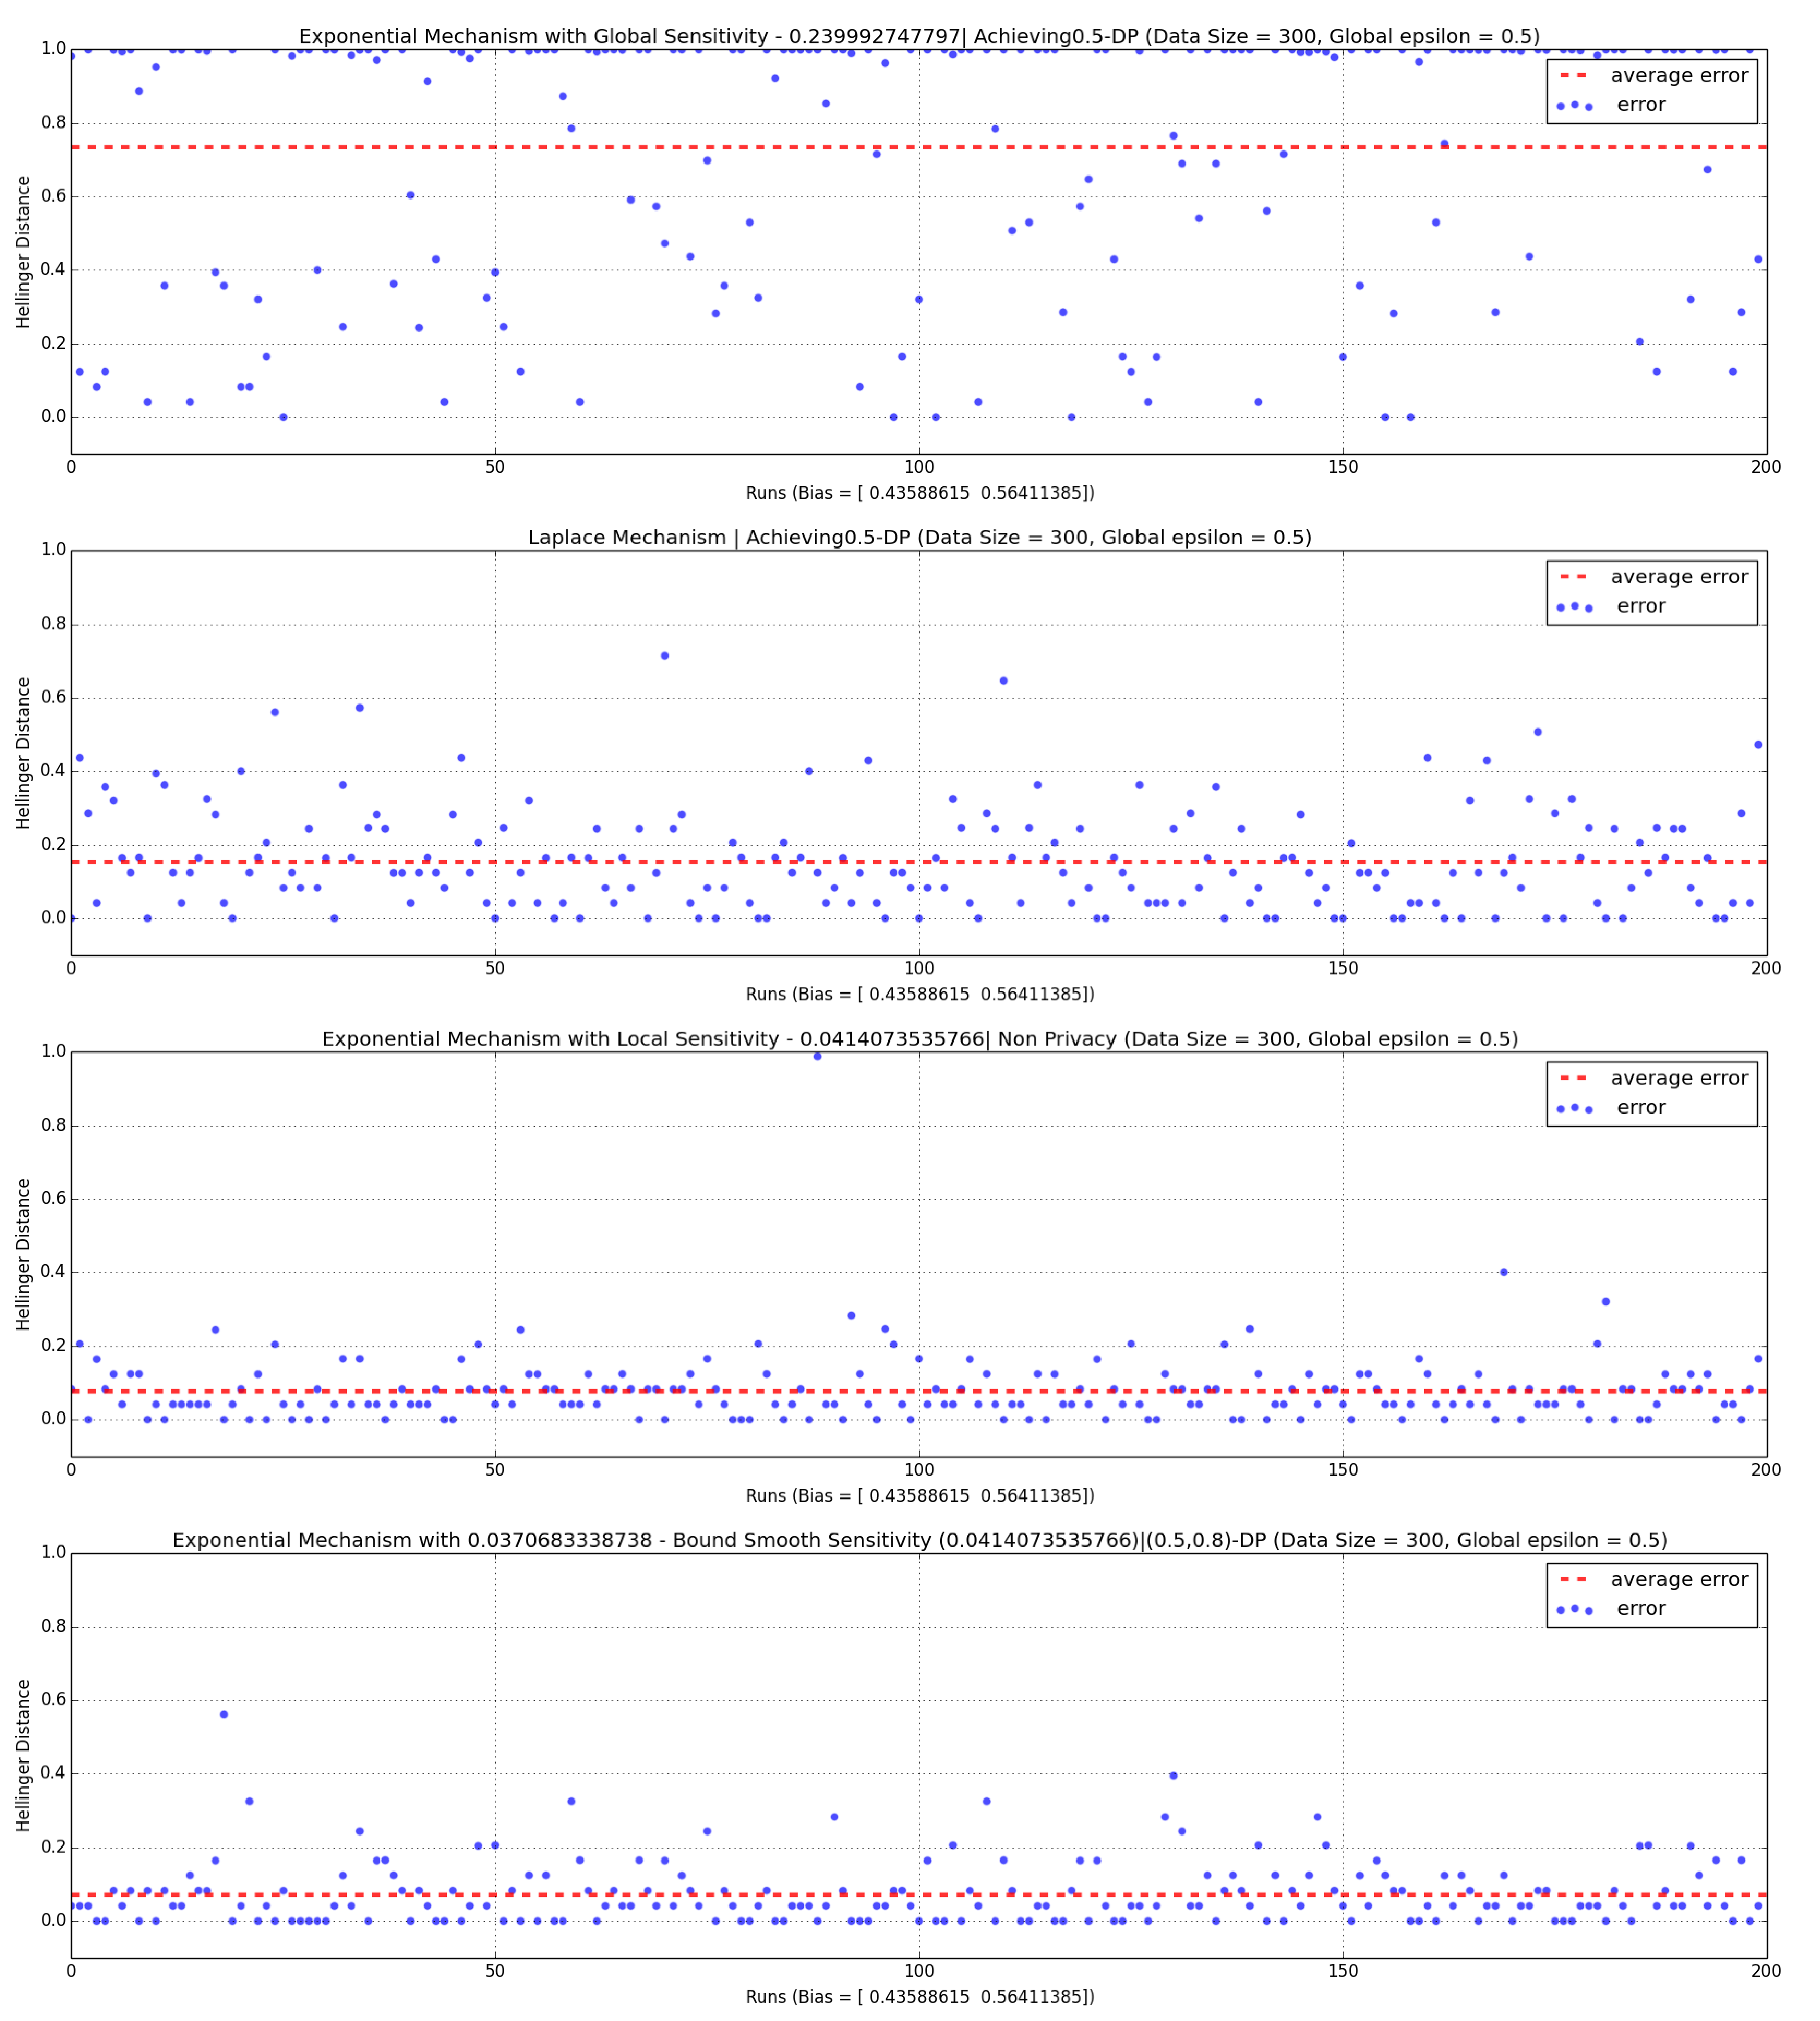
\includegraphics[width=0.48\textwidth]{accuracy_1.eps}}
%   \subfigure[Data size $n = 200$ with global $\epsilon = 0.8$]{
%     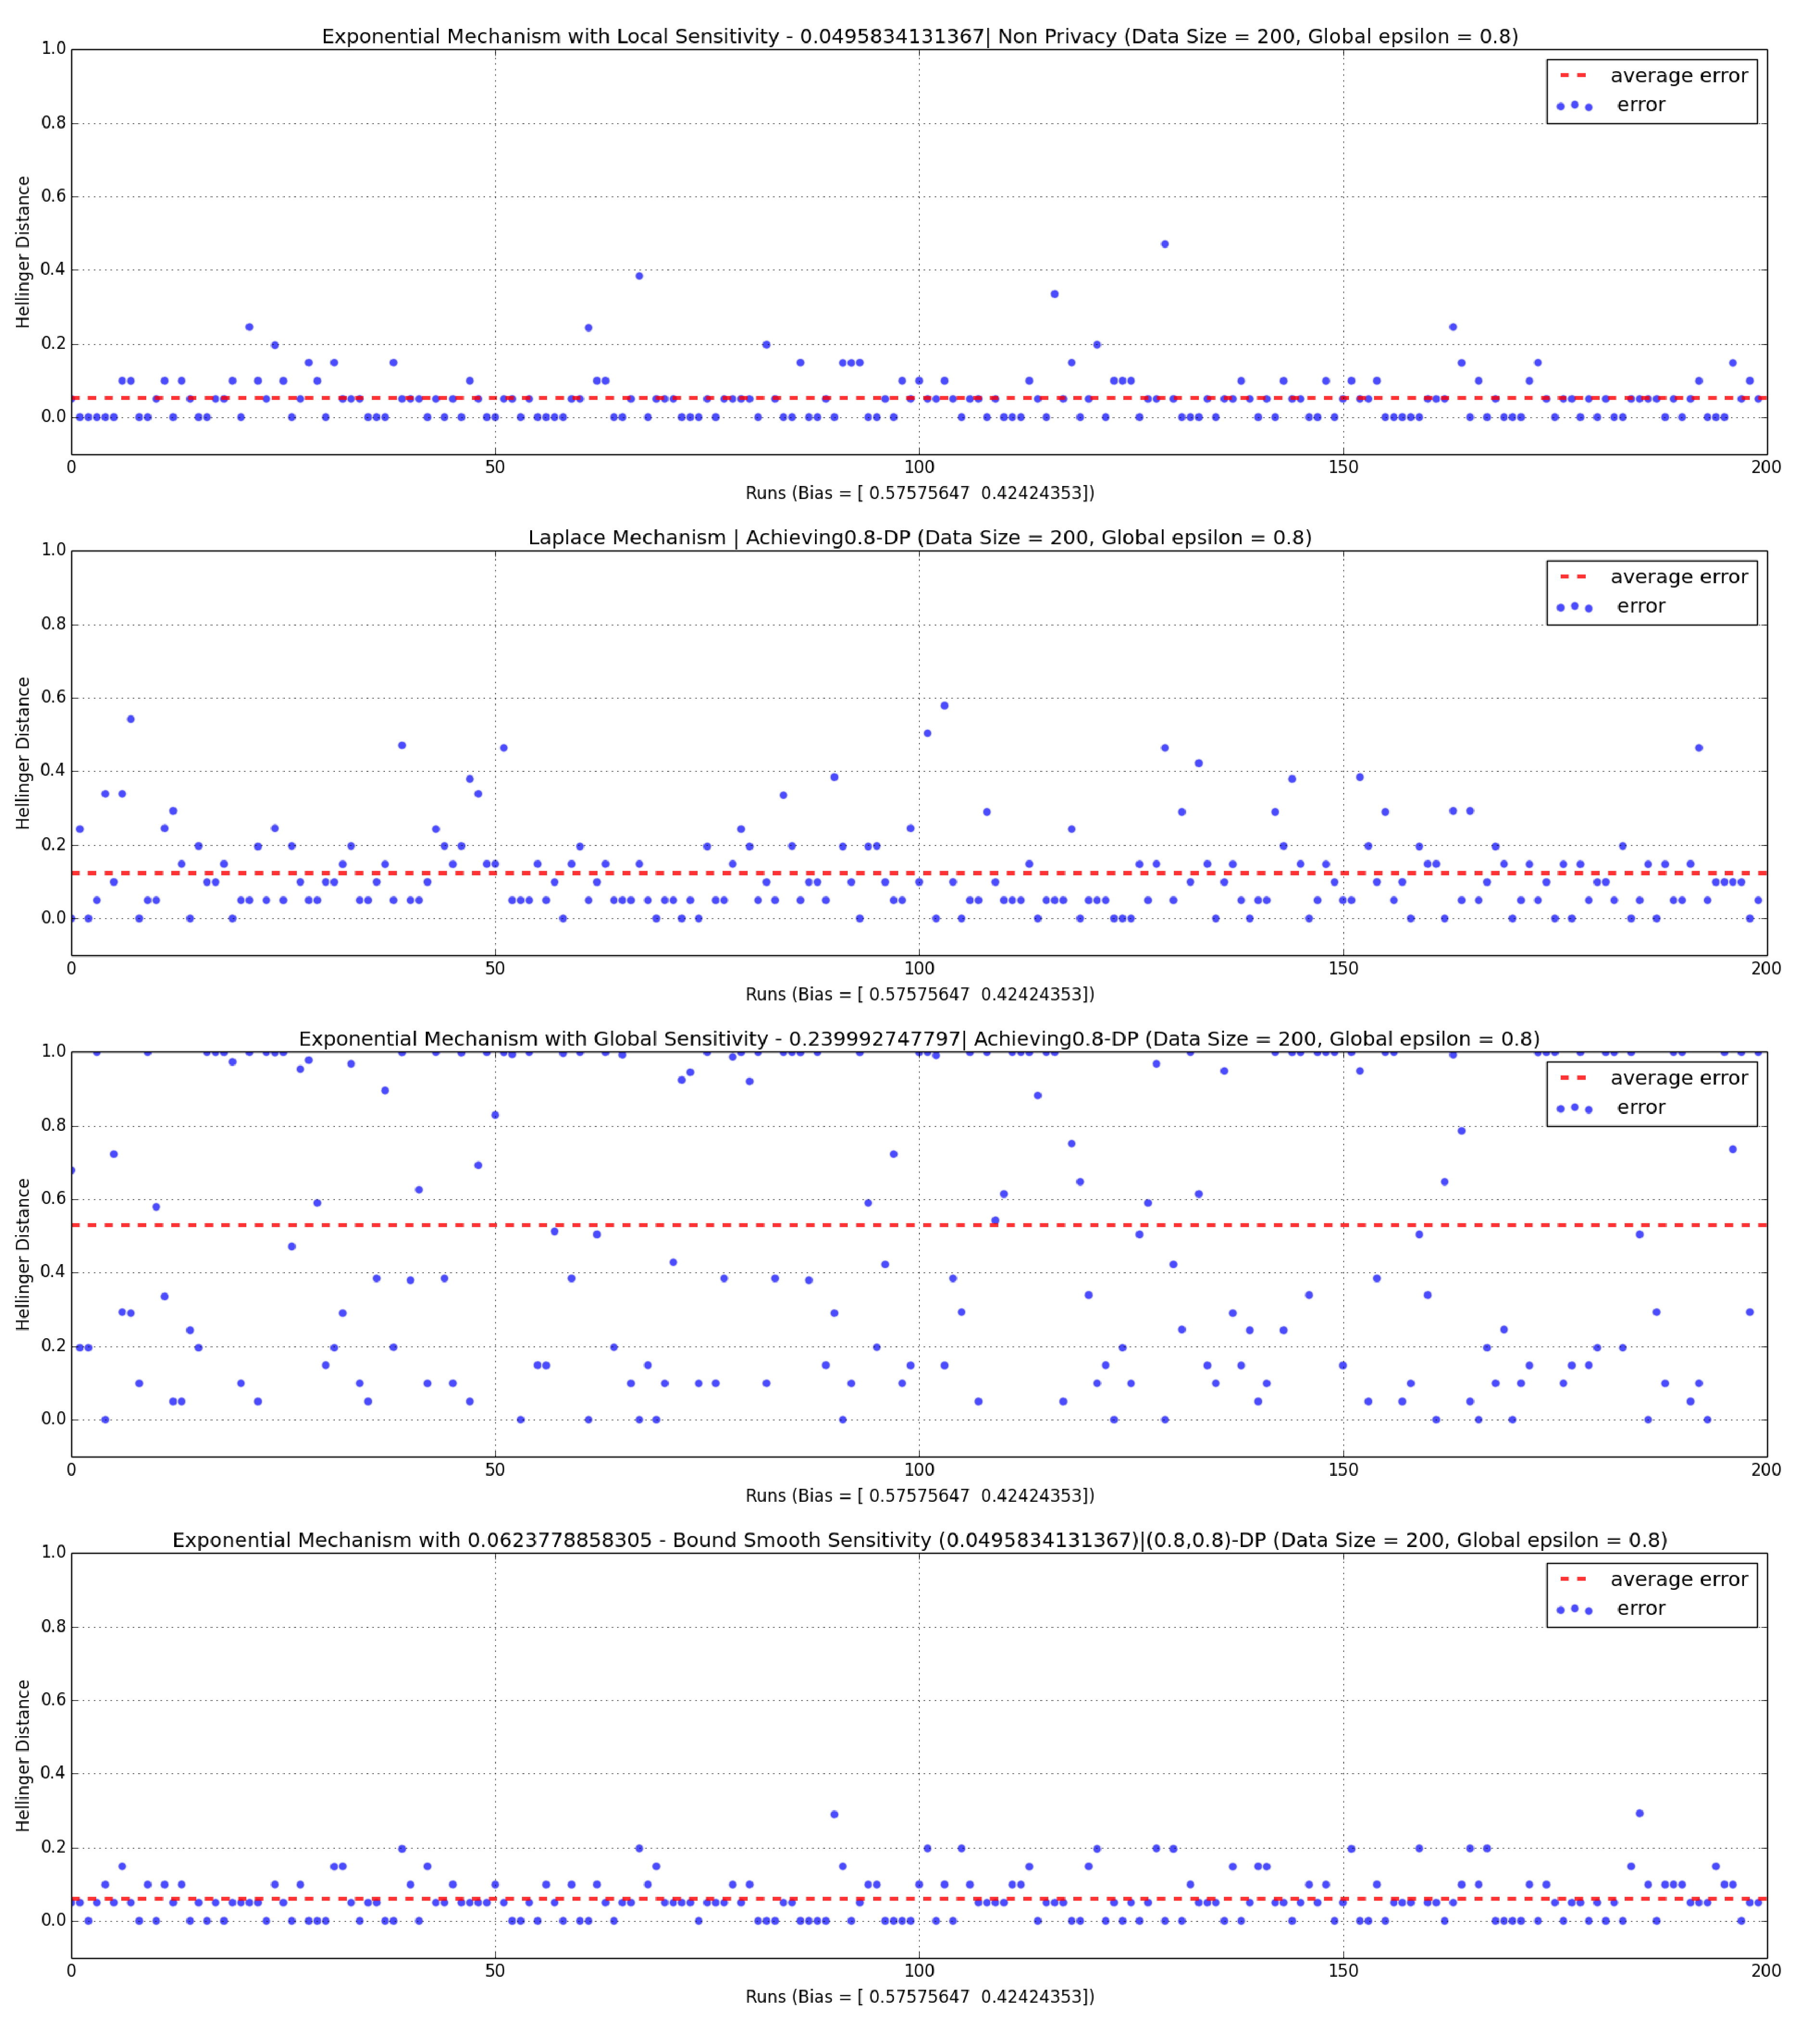
\includegraphics[width=0.48\textwidth]{accuracy_2.eps}} 
% \caption{The experimental results of accuracy of four algorithms}
% \label{fig_data}
% \end{center}
% \end{figure*}

We first analyzed the accuracy based on the Hellinger distance. By repeating the experiments for 10000 times and plotting the accuracy of each execution, we got two groups of results under different parameters setting as in Fig. \ref{fig_beta_hellinger} and Fig. \ref{fig_dirichlet_hellinger}. X-axis is labeled with different mechanisms. We took four mechanisms in our experiments: our newly designed exponential mechanism with smooth sensitivity named ``ExpoMech of SS'', exponential mechanism with local sensitivity named `` ExpoMech of LS'', exponential mechanism with global sensitivity named `` ExpoMech of GS'' and Laplace mechanism named ``LaplaceMech''. Y-axis is the accuracy measured by Hellinger distance between output $z$ of each execution and the correct inference result $\bysinfer(x)$, $\hlg(z, \bysinfer(x))$.

When prior distribution is $\betad$, under data size $n = 500$ and $300$, we obtained two plots in Fig. \ref{fig_beta_hellinger}. It is shown that our ExpoMech of SS is slightly better than Laplace mechanism and much more better than it with global sensitivity.

To have more experimental results, we then extended the $\betad$ to the Dirichlet distribution $\dirichlet$ as well as increased the data size, plotted in Fig. \ref{fig_dirichlet_hellinger}.

Then, we study the accuracy of these four mechanisms based on $l_1$ norm, with the Dirichlet distribution $\dirichlet(7,4,5)$ and data size $150$ for comparison, as in Fig. \ref{fig_dirichlet_hellinger_l1}.

The results based on $l_1$ norm are actually very similar to results based on Hellinegr distance.


In both of the two cases, the performances of our exponential mechanism with smooth sensitivity and Laplace mechanism are very close. 

\section{Conclusions}
We can obtain some preliminary conclusions: 
\begin{enumerate}
	\item Our exponential mechanism with smooth sensitivity can have similar accuracy as it with local sensitivity. Both of the two exponential mechanisms are do much better than it with global sensitivity.
	\item The accuracy of our exponential mechanism is better than Laplace mechanism. But the advantages are not significant.
\end{enumerate} 

In consequence, we have a further experiments exploration on the accuracy trade-off between Laplace mechanism and our exponential mechanism in next section.


\bibliographystyle{plain}
\bibliography{bayesian.bib}

\end{document}

